\chapter{Chip Design}\label{chap:sysdes}

	The required functionality of the chip can be realized in many ways. This chapter aims at explaining and choosing an appropriate setup of sub-circuits given the requirements from SAAB.

	\section{Overall performance}
		The required performance of the down-converter is listed in \autoref{app:specs}. These specifications list requirements that the chip is expected to achieve. Besides these there is a list for targeted performance. That is, a list of important parameters of the chip that should be improved upon given the possibility. These are the bandwidth, the noise, the linearity and the gain. The chip design takes all these parameters into account.

		A system's noise and linearity are counterparts. To see this dualism, a two-component system composed of a component with low attenuation and an amplifying component is considered. If the amplifier is placed before the attenuator the overall noise figure ($\nf$) of the system will be approximately the few decibels of noise present in the amplifier. The $IIP_3$ will on the other hand be limited by the output power of the amplifier. In a reversed system, with the attenuator first, the $\nf$ will become the loss in the attenuator plus the noise in the amplifier. The $IIP_3$ however, will be higher, benefiting from the initial loss according to \autoref{eq:casciip3}.

		Naturally there is a minimum of components necessary to achieve the specified performance. The mixing circuit needs a dedicated amplifier to amplify the LO-signal to an appropriate power level. Unless an image reject mixer is used, there is a need for a filter to remove the image frequencies which taint the signal. The RF-to-IF chain needs amplifiers and a variable attenuator block. The nominal chip gain is set to be \unit[8--10]{dB} with a $\unit[\pm 5]{dB}$ gain control. This means that the signal must be amplified at least \unit[13]{dB} plus losses in the entire circuit. If the losses in the mixer and the attenuator block are \unit[10]{dB}, then the gain of the amplifiers must be at least \unit[23]{dB}.

	\section{Component performance}
		To estimate the performance of different layouts, typical performances of the individual components are needed. However, as this is an analysis made prior to the design, the performances are only estimated. In \autoref{tab:compperformance} the estimates are presented.

		\begin{table}[hbt!]
			\caption[Estimated performance of chip components.]{Estimated performance of the chip's components.}
			\label{tab:compperformance}
			\centering
			\begin{tabular}{ l l l l } \toprule
				& Mixer & Amplifier & Attenuators \\\midrule
				Gain & \unit[-8]{dB} & $\unit[<13]{dB}$ & \unit[-2--12]{dB} \\
				$\nf$ & \unit[8]{dB} & \unit[1--2]{dB} & \unit[2--12]{dB} \\
				$IIP_3$ & \unit[20--27]{dBm} & \unit[14--22]{dBm} & \unit[30]{dBm} \\\bottomrule
			\end{tabular}
		\end{table}

		The mixer losses are due to the two sidebands and to the reactive circuits. The inherent splitting of the signal into two sidebands effectively reduces the gain with \unit[3]{dB} (\autoref{sec:mixer_introduction}). Depending on the type of mixer, the losses in the filters and/or baluns usually amount to about \unit[3--7]{dB}, depending on complexity. The estimates are based on the properties of resistive mixers. As explained in \autoref{sec:fet_mixers}, a resistive mixer is chosen since they are very linear. The $IIP_3$ of a mixer is the most difficult property to estimate. One of the main topics of the thesis is to evaluate the linearity of different mixer topologies. The estimate used here for mixer $IIP_3$ (\unit[25]{dBm}) as well as for losses in diplexer and mixer (\unit[8]{dB}) are taken from the initial mixer study reported in \autoref{ch:mixer}.

		UMS, the foundry producing the MMIC chips, have amplifiers in PPH25 with an unconditionally stable gain up to about \unit[13]{dB}, depending on the other characteristics.\autocite{pph25manual}

		Attenuator blocks from previous works have been studied and even though there are different ways to realize them, the performances are more or less the same.\autocite{gustavsson07}

	\section{Budget analysis}\label{sec:budget_analysis}
		The purpose of the budget analysis is to estimate the performance of the MMIC based on the estimates made of each individual component. With the noise target $\nf<\unit[12]{dB}$ and linearity target $IIP_3>\unit[17]{dBm}$, it is evident that the priority is high linearity and that the signal chain thus needs to start with an attenuating device. All components placed before the mixer in the signal path need to have a \unit[0.5]{GHz} bandwidth while components placed after only need performance for a \unit[20]{MHz} narrow band. Estimates of full chip performance are made for some different component permutations at different gain states. This way, the effect on the performance due to different gain settings is taken into account.

		The performance of a chip layout starting out with the gain block (\autoref{tab:confper2}) has two inherent problems. The first is that all components prior to the mixer must be wideband and the second is that the entire chip performance becomes sensitive to the gain setting (compare with \autoref{tab:confper1}). Due to these, only chip layouts starting out with the mixer are considered feasible. Also, if the mixer is placed first, there are possibilities to integrate the filter with the input networks existing in most mixer designs.
		
		\begin{table}[hpt!]
			\caption[Estimated performance of chip setup 2.]{Estimated performance of chip setup 2. The order of the components is: Filter, attenuators, amplifier, mixer and amplifier.}
			\label{tab:confper2}
			\centering
			\begin{tabular}{ l l l l }
				\multicolumn{4}{c}{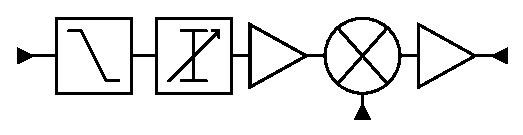
\includegraphics[width=0.6\textwidth]{fig/system/sys2}} \\\toprule
				& Nominal gain & Gain: \unit[+5]{dB} & Gain: \unit[-5]{dB} \\\midrule
				Gain & \unit[9]{dB} & \unit[14]{dB} & \unit[4]{dB} \\
				$\nf$ & \unit[12.0]{dB} & \unit[7.0]{dB} & \unit[17.0]{dB} \\
				$IIP_3$ & \unit[18.4]{dBm} & \unit[13.6]{dBm} & \unit[22.8]{dBm} \\\bottomrule
			\end{tabular}
		\end{table}

		\begin{table}[hpt!]
			\caption[Estimated performance of chip setup 1.]{Estimated performance of chip setup 1. The order of the components is: Filter, mixer, amplifier, attenuators and amplifier.}
			\label{tab:confper1}
			\centering
			\begin{tabular}{ l l l l }
				\multicolumn{4}{c}{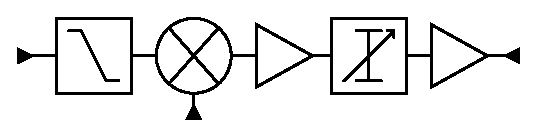
\includegraphics[width=0.6\textwidth]{fig/system/sys1}} \\\toprule
				& Nominal gain & Gain: \unit[+5]{dB} & Gain: \unit[-5]{dB} \\\midrule
				Gain & \unit[9]{dB} & \unit[14]{dB} & \unit[4]{dB} \\
				$\nf$ & \unit[10.7]{dB} & \unit[10.0]{dB} & \unit[12.4]{dB} \\
				$IIP_3$ & \unit[18.5]{dBm} & \unit[16.4]{dBm} & \unit[19.4]{dBm} \\\bottomrule
			\end{tabular}
		\end{table}
		
		\begin{table}[hpt!]
			\caption[Estimated performance of chip setup 3.]{Estimated performance of chip setup 3. The order of the components is: Filter, mixer, amplifier, amplifier and attenuators.}
			\label{tab:confper3}
			\centering
			\begin{tabular}{ l l l l }
				\multicolumn{4}{c}{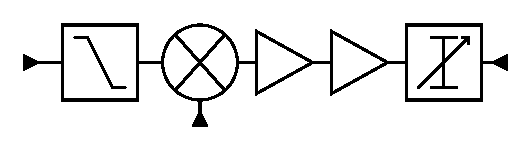
\includegraphics[width=0.6\textwidth]{fig/system/sys3}} \\\toprule
				& Nominal gain & Gain: \unit[+5]{dB} & Gain: \unit[-5]{dB} \\\midrule
				Gain & \unit[9]{dB} & \unit[14]{dB} & \unit[4]{dB} \\
				$\nf$ & \unit[9.9]{dB} & \unit[9.9]{dB} & \unit[10.1]{dB} \\
				$IIP_3$ & \unit[10.5]{dBm} & \unit[10.5]{dBm} & \unit[10.5]{dBm} \\\bottomrule
			\end{tabular}
		\end{table}

		\begin{table}[hpt!]
			\caption[Estimated performance of chip setup 4.]{Estimated performance of chip setup 4. The order of the components is: Filter, mixer, attenuators, amplifier and amplifier.}
			\label{tab:confper4}
			\centering
			\begin{tabular}{ l l l l }
				\multicolumn{4}{c}{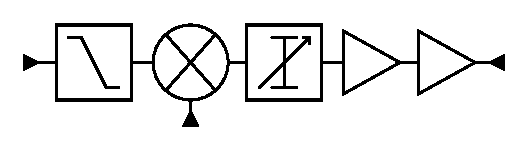
\includegraphics[width=0.6\textwidth]{fig/system/sys4}} \\\toprule
				& Nominal gain & Gain: \unit[+5]{dB} & Gain: \unit[-5]{dB} \\\midrule
				Gain & \unit[9]{dB} & \unit[14]{dB} & \unit[4]{dB} \\
				$\nf$ & \unit[16.9]{dB} & \unit[11.9]{dB} & \unit[21.9]{dB} \\
				$IIP_3$ & \unit[21.4]{dBm} & \unit[18.0]{dBm} & \unit[23.4]{dBm} \\\bottomrule
			\end{tabular}
		\end{table}

		Considering the three setups starting with a mixer, the layout in \autoref{tab:confper3} gives a good noise figure but too low $IIP_3$ and the layout in \autoref{tab:confper4} gives high $IIP_3$ but too much noise. The layout in \autoref{tab:confper1}, starting out with a mixer and then alternating amplifier and attenuator, gives the best trade-off in performance and low sensitivity to different gain states. With this design, it should be possible to reach the required performance as stated in the specifications. Also, the targeted performance will be met at most gain states.

	\section{Realization}
		The components are designed individually based on the above plan. Specific performance demands on individual components are discussed in depth in each section. The report is segmented to separate different classes of components such as amplifiers and mixers into different chapters.

		The mixer circuit and the image reject low-pass filter are detailed in \autoref{ch:mixer}. It starts out with a theoretical treatment of the mixing process and the importance of the LO drive. Decisions regarding topology and other design aspects follow. The design of a FET-mixer is then reported along with simulated results.

		Three different types of amplifiers are designed and reported in \autoref{ch:amp}. The first one is the LO-amplifier running in compression to provide an amplified and stable LO signal to the mixer. The second and third amplifiers are placed on the IF path, to provide the necessary chip gain. The first is designed to minimize the noise contribution while the second is designed to maximize power output and thereby chip linearity.

		In \autoref{ch:vargain} are the design and results of a variable attenuator block explained. This block is needed to control the chip gain.

	\newpage
	\section{Comparison to final result}
		The figures above are based on prior estimates. \autoref{tab:confper1final} lists the results achieved with the layout in \autoref{tab:confper1} and shows a good agreement.

		\begin{table}[hpt!]
			\caption[Achieved simulated performance with chip setup 1.]{Achieved simulated performance with chip setup 1. The results are in agreement with the prior estimates detailed in \autoref{tab:confper1}.}
			\label{tab:confper1final}
			\centering
			\begin{tabular}{ l l l l }
				\multicolumn{4}{c}{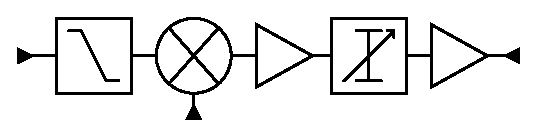
\includegraphics[width=0.6\textwidth]{fig/system/sys1}} \\\toprule
				& Nominal gain & Gain: \unit[+4.4]{dB} & Gain: \unit[-6]{dB} \\\midrule
				Gain & \unit[10.6]{dB} & \unit[15.0]{dB} & \unit[4.6]{dB} \\
				$\nf$ & \unit[11]{dB} & \unit[10]{dB} & \unit[13]{dB} \\
				$IIP_3$ & \unit[20]{dBm} & \unit[17]{dBm} & \unit[21]{dBm}  \\\bottomrule
			\end{tabular}
		\end{table}
